%%=============================================================================
% Создавайте лекции, используя этот шаблон. Не забывайте удалять из шаблона
% лишние комментарии.
% Шаблон начинается с указания класса lecture-notes.
%%=============================================================================
\documentclass[russian]{lecture-notes}

\usepackage[final]{graphicx}
\usepackage{amsmath}
\usepackage{svg}
\usepackage{timestamps}

\title{Рекуррентные тропические последовательности}
\author{Составили: Лукашов Никита, Смирнова Вероника, Беляева Анна}
\date{}

\begin{document}
\youtubevideo{zIYfYT5THDY}

\maketitle
\timestamp{00:00}
\section{Классические рекуррентные последовательности}

 Сначала мы рассмотрим классические рекуррентные последовательности, для которых уже есть завершённая теория, а затем перейдём к тропическим.
\timestamp{00:45}
\subsection{Что такое классическая реккурентная последовательность?}

\begin{Definition}
	Пусть дан вектор $ a=(a_0,\ldots, a_n) \in \mathbb{R}^{n+1}, a_0 \ne~0, a_n \ne~0$
	Тогда последовательность $\{z_{i}\}_{i\in \mathbb{Z}}$ называется рекуррентной последовательностью, удовлетворяющей вектору $a$, если для $ \forall k \in \mathbb{Z} $ выполнено следующее условие:
	\[
	\sum_{0\le i \le n}a_iz_{k+i}=0
	\]
\end{Definition}

Если вектор $a$ фиксированный, то это~--- линейное условие на $z$.


 Замечательное свойство состоит в следующем: если последний коэффициент $a_n$ не равен нулю и если мы вычислили, допустим, все $z$ до какого-то $z_i$, то $z_{i+1}$ мы можем однозначно вычислить, подставив в формулу соответствующее $k$.

Пример:

1) Числа Фибоначчи:

$a=(1, 1, -1), z_{k+2}=z_{k+1}+z_k \; (z_0=0, z_1=1)$

Это формула числа кроликов в очередном поколении: число кроликов в следующем поколении ~--- это число в текущем плюс в предыдущем.

Далее по этой формуле можно вычислять каждое число однозначным образом.
\timestamp{04:00}
\subsection{Описание рекуррентной последовательности, удовлетворяющей вектору $a$}

\begin{Definition}
	Многочлен $f$ от переменной $x$ называется характеристическим многочленом рекуррентной последовательности, если
	\[
	f=\sum_{0\le i \le n}a_ix^i
	\]
	Коэффициенты этого многочлена ~--- это координаты вектора $a$.
	\vspace{\baselineskip}
\end{Definition}


\begin{Theorem}
	Если $x$ ~--- корень характеристического многочлена рекуррентной последовательности, то последовательность \{$z_i=x^i\}_{i\in \mathbb{Z}}$ удовлетворяет вектору $a$. Если $x$ - кратный корень многочлена, то необходимо взять производную: $\{z_i=ix^{i-1}\}_{i\in \mathbb{Z}}$ Если кратность корня равна $m$, то нужно взять $0, 1, \ldots, m-1$ производные $x^i$. Все эти последовательности будут удовлетворять рекуррентному соотношению.
\end{Theorem}


 Пониманию второй части теоремы поможет следующая лемма.\\
\begin{Lemma}
	Если многочлен $P(x)$ имеет корень $x=a$ кратности $k$, то $P'(x)$ имеет корень $x=a$ кратности $k-1$.
\end{Lemma}



\emph{Примеры:}
\begin{enumerate}

\item Дан вектор $a=(1, -2, 1)$

 Это означает, что $z_{k+1}=2z_k-z_{k-1}$

 Тогда характеристический многочлен $f=x^2-2x+1=(x-1)^2$ имеет кратность 2.

 Рекуррентная последовательность, удовлетворяющая вектору $a$, выглядит так:

 $z_i=x^i|_{x=1}=1$

 Последовательность, состоящая из единиц, удовлетворяет этому вектору:

$1-2+1=0$

 Но поскольку корень имеет кратность 2, можно построить другую последовательность:

 $z_i=ix^{i-1}|_{x=1}=i:$

$..., -2, -1, 0, 1, 2, 3, \dots$

Проверим, что она удовлетворяет вектору $a$ в произвольном месте:

$1*(-2)-2*(-1)+0=0$

Действительно, последовательность удовлетворяет вектору $a$. \\

\item Дан вектор $a=(-12, 16, -7, 1)$

Это означает, что $-12z_{k-2}+16z_{k-1}-7z_{k}+z_{k+1}=0$

Тогда характеристический многочлен $f=x^3-7x^2+16x-12=(x-2)^2(x-3)$ имеет два корня, один из которых ($x=2$) имеет кратность 2.
Рекуррентные последовательности,удовлетворяющие вектору $a$:
\end{enumerate}

1)$z_i=x^i|_{x=3}=3^i:$


$..., 1, 3, 9, 27, 84, ...$

Проверим, удовлетворяет ли эта последовательность

вектору $a$ в произвольном месте:

$-12*1+16*3-7*9+27=0$

Значит, последовательность удовлетворяет вектору $a$.

2) $z_i=x^i|_{x=2}=2^i$

$..., 1, 2, 4, 8, 16, ...$

Аналогично проверим:

$ -12*1+16*2-7*4+8=0$

Значит, последовательность удовлетворяет вектору $a$.

3)Поскольку корень $x=2$ имеет кратность 2, можно

построить другую последовательность:

$z_i=ix^{i-1}|_{x=2}=i*2^{i-1}:$

$..., 0, 1, 4, 12, ...$

Проверка:

$0+16*1-7*4+12=0$

Аналогично, последовательность удовлетворяет вектору $a$.
\\
\timestamp{09:35}
\begin{Theorem}
	n рекуррентных последовательностей, соответствующие корням характеристического многочлена с нужными кратностями, составляют базис линейного пространства всех рекуррентных последовательностей, которые удовлетворяют вектору $a$. Это пространство имеет размерность n, а корни характеристического многочлена и их производные ~--- его базис.
	\label{Theorem_2}
\end{Theorem}


 То есть, рекуррентные последовательности, образующие линейнoе пространство, можно складывать между собой и умножать на произвольное число.


\emph{Пример:}

 Проиллюстрируем теорему на числах Фибоначчи:

Характеристический многочлен имеет вид: $x^2-x-1$

 Он имеет два корня: $x_1=\frac{1+\sqrt{5}}{2}$ \; (золотое сечение) и $x_2=\frac{1-\sqrt{5}}{2}$

 По \ref{Theorem_2}, имеем две базисные  последовательности: $z^{(1)}_i=x^i_1, z^{(2)}_i=x^i_2: \; i\in \mathbb{Z}$

Это иррациональные числа. Чтобы получить целые, необходимо выполнить следующую комбинацию: $\frac{(x^i_1-x^i_2)}{\sqrt5}$. Это формула и является явной формулой для вычисления $i$-ого члена последовательности чисел Фибоначчи.
\timestamp{00:00}
\section{Основные понятия в тропической алгебре}

\timestamp{14:40}
\subsection{Тропические объекты}

Основным объектом тропической математики является \emph{тропическое полукольцо}  (обозначим его как $T$).
\addcontentsline{toc}{subsection}{2.2. Тропические объекты}

Если $T$ ~---  упорядоченная полугруппа, то $T$ ~--- это тропическое полукольцо, в котором в качестве базисных определено две операции: $\oplus :=min$ (то есть мы можем сказать, какой из двух элементов меньше) и $ \otimes :=+ $ (обычная операция сложения в полугруппе).

Если $T$ ~--- упорядоченная группа, то $T$ ~--- это тропическое полуполе с ещё одной операцией тропического деления $\oslash:= - $ (обычная операция вычитания в группе). Настоящего вычитания нет, так как операции, обратной взятию минимума, не существует.

Итак, в тропической алгебре есть сложение как минимум, умножение как сложение и деление как вычитание.


Примеры:
\begin{enumerate}
	\item $\mathbb{Z}^+=\{0\le a \in \mathbb{Z}\}$ - целые неотрицательные числа;
	\item $\mathbb{Z}^+_\infty= \mathbb{Z}^+\cup \{\infty\}$ - целые неотрицательные числа, к которым добавлена бесконечность.
	Оба этих примера являются тропическими коммутативными полукольцами.
	\\

	При этом бесконечность на тропическом языке играет роль нуля, а ноль - единицы:

	$ a \oplus \infty=min\{a, \infty\}=a $

	$a \otimes \infty=a+\infty=\infty$
	$a \otimes 0=a+0=a$
	\item $\mathbb{Z}, \mathbb{Z}^\infty$ - тропические полуполя.
	\item Матрицы $n\times n$ над полуполем $\mathbb{Z}^\infty$ образуют некоммутативное тропическое полукольцо:
	$(a_{ij})\otimes (b_{kl})=(\oplus_{1\le j\le n}a_{ij}\otimes b_{jl})$ (здесь умножение матриц переписано в тропических терминах)
\end{enumerate}


\timestamp{20:00}
\subsection{Тропические многочлены}

\begin{Definition}
	Моном $Q=a\otimes x_1^{\otimes i_1}\otimes\ldots\otimes x_n^{\otimes i_n}$ называется тропическим, где $x^{\otimes i}=x\otimes\ldots\otimes x$, его тропическая степень равна $trdeg=i_1+\ldots+i_n$. Тогда в классическом виде: $Q=a+i_1x_1+\ldots+i_nx_n$ - обычная линейная функция.
	\end{Definition}
\timestamp{21:20}
\begin{Definition}
	Полином $f=\oplus_j(a_j\otimes x_1^{i_{j1}}\otimes\ldots\otimes x_n^{i_{jn}})=min_j\{Q_j\}$ является тропическим. В классическом виде он представляет собой минимум линейных функций.
		\end{Definition}


 Полином представляет собой выпуклую кусочно-линейную функцию:


\begin{figure}[h!]
\center{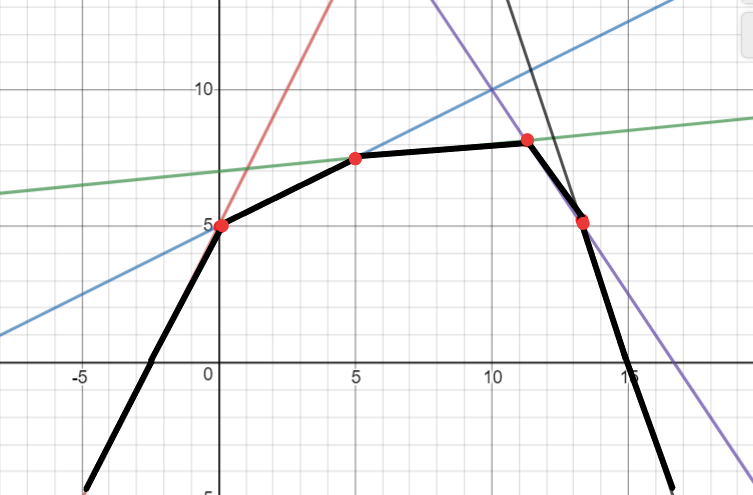
\includegraphics[scale=0.4]{tempsnip.png}}
\caption{Минимум линейных функций}
\end{figure}
\begin{Definition}
	Минимум линейных функций - это выпуклая кусочно-линейная функция, любое значение которой является наименьшим из значений $y$ таких, что пара $(x,y)$ лежит на одной из заданных функций.\\
	\end{Definition}
\timestamp{25:30}
\begin{Definition}
Вектор $x=(x_1,\ldots, x_n)$ - тропический корень многочлена $f$, если минимум $min_j\{Q_j\}$ достигается по крайней мере на двух разных мономах, на двух разных значениях j.
\end{Definition}
Так, например, на Рис.1 видно, у такого тропического полинома 4 корня.

Чем примечательна кусочно-линейная функция? Там, где она линейна, она дифференцируема. А там, где она ломается, она не дифференцируема, не гладкая. Иными словами можно сказать, что тропический корень - это то место, где функция не гладкая.
\timestamp{29:00}
\subsection{ Тропические линейные системы}

\begin{Definition}
	$min_{1\le j\le n}\{a_{i,j}+x_j\}, 1\le i\le m$ (или $(m\times n)$ - матрица $A=(a_{i,j})$, так как здесь $n$ переменных и $m$ уравнений) ~--- тропическая линейная система.
	\end{Definition}
\timestamp{00:00}
\begin{Definition}
	Аналогично, вектор $x=(x_1,\ldots, x_n)$ является решением тропической линейной системы, если в каждой строчке $1\le i\le m$ найдутся два столбца $1\le k<l\le n$ такие, что:
	\[
	a_{i,k}+x_k=a_{i,l}+x_l=min_{1\le j\le n}\{a_{i,j}+x_j\}
	\]
	\end{Definition}


\timestamp{35:55}
\section{Тропические рекуррентные последовательности}
\begin{Definition}
	Пусть есть вектор $a=(a_0,\ldots ,a_n)\in (\mathbb{R} \cup \{\infty\})^{n+1}, a_0<\infty , a_n<\infty$. Тогда $y=\{y_i\in \mathbb{R}\cup \{\infty\}\}_{i\in\mathbb{Z}}$ - тропическая рекуррентная последовательность, удовлетворяющая вектору $a$, если для любого $k\in\mathbb{Z}$ выполнено линейное тропическое уравнение:
	\[
	min_{0\le i\le n}\{a_i+y_{k+i}\}
	\]
\end{Definition}
\bfseries Определение: \mdseries


Тропические линейные последовательности, удовлетворяющие $a$, образуют линейное пространство $R_a$: если $y, z \in R_a $, то для $b, c\in \mathbb{R}\cup\{\infty\}$
\[
b\otimes y\oplus c\otimes z=\{min\{y_i+b, z_i+c\}\}_{i\in\mathbb{Z}}\in R_a
\]

Замечание: если в классических рекуррентных последовательностях каждый член вычислялся однозначно, то в тропических это не всегда так.


Пример:

Пусть $n=2, a=(a_0, a_1, a_2).$
Необходимо, чтобы минимум достигался два раза. Здесь может быть две разных ситуации:

%%%%%%%
%%%%%
%%%
Согласно последовательности $
 \ldots y_0,\:y_1,\:y_2,\ldots,\:y_i,\:y_{i+1},$
где мы уже построили $y_0,\:y_1,\:y_2,\ldots,\:y_i.$, а $y_{i+1}$ ~--- неизвестное, мы должны написать такое уравнение
\[
a_0+y_{i-1},\:a_1+y_i,\:a_2+y_{i+1},
\]


где $a_2+y_{i+1}$-неизвестное.
\vspace{\baselineskip}

\begin{enumerate}
 \item   Допустим, что минимум мы обозначили из предыдущих двух
$$m=min\{{a_0+y_{i-1},a_1+y_i}\},$$

и он достигается на предыдущей последовательности один раз. Это значит, что минимум, например, равен первому члену, но поскольку минимум достигается один раз, то он строго меньше второго
$$m=a_0+y_{i-1}<a_1+y_i$$

или, наоборот, минимум достигается на втором члене и он меньше первого
$$m=a_1+y_i<a_0+y_{i-1}$$

Тогда для удовлетворения уравнения \ref{1} минимум должен быть достигнут на последнем члене. Мы получаем, что
$$a_2+y_{i+1}=m$$

Отсюда однозначно вычисляем $y_{i+1}=m-a_2$.

Эта ситуация была <<хорошей>>, то есть следующий член вычисляется однозначно.

 \item  Допустим, минимум достигался два раза и был равен и тому, и другому члену
$$m=a_0+y_{i-1}=a_1+y_i.$$

И тогда оказывается, что у нас бесконечно много возможностей. Мы можем написать, что $a_2+y_{i+1}\geq m.$
Или, переписав, получаем
$$y_{i+1}\geq m-a_2$$
-- мы можем взять любое число на этом луче.

Получается луч возможностей для $y_{i+1}$, для которого мы можем взять произвольное число. Вследствие этого однозначность теряется.
\end{enumerate}

В этом и заключается трудность вычисления тропических рекуррентных последовательностей, потому что иногда может случиться, что у нас есть бесконечно много возможностей, и мы должны их все учесть. Потом на следующем шаге опять может случиться,  что у нас есть
единственная возможность, а может ~--- бесконечно много возможностей.

В этом состоит принципиальное отличие от классической ситуации.



 Примеры:
\begin{enumerate}
 \item
\slshape$a=(0,0)$, тогда рекуррентная последовательность $\{y_i=0\} _{i\in Z}$ удовлетворяет $a$.\upshape

Данная ситуация еще проще, ведь членов последовательности всего два. Тогда, например, рекуррентная последовательность, которая состоит из нулей, будет удовлетворять $a$: $min\{0+0,0+0\}=0$ и так бесконечно много раз.\

Легко заметить, что данному вектору будет удовлетворять любая последовательность, состоящая из одинаковых чисел.
Возьмем $\{y_i=1\} _{i\in Z}$, тогда $min\{0+1,0+1\}=1$. Или $\{y_i=c\} _{i\in Z}$,
тогда $min\{0+c,0+c\}=c$.

\item
Когда последовательность
длины менее 2, т.е. n=1 - это уже простая однозначная последовательность. Мы каждый следующий член
вычисляем единственным образом.

Но, начиная с двойки, мы видим, что
возникает неоднозначность.

\item

$a=(0,0,0).$ Возьмём набор $I=\{\ldots ,<i_{-1}<i_0<i_1<\ldots \}, i_{j+1}-i_j\geq 3$ и рекуррентная последовательность $\{y_i=0, i\notin I, y_i\geq 0, i\in I\}$ удовлетворяет $a$.


Пусть а состоит из трех нулей. Что мы можем сделать? Появляется неограниченное число возможностей. Выберем какие-то  индексы $i_{-1},i_0,i_1$. Единственное ограничение, чтобы разность
между двумя соседними была не меньше трех. Можем взять в качестве набора I арифметическую прогрессию: 0, 3, 6 ,9 и т.д. И тогда рекуррентную последовательность, удовлетворяющую а, можно взять таким образом: берём на всех местах, вне этого множества I, нули, а на выделенных  местах i берем что-то не отрицательное, т.е. произвольное.

Любая такая последовательность будет удовлетворять а, потому что здесь появляется <<дыра>> между соседними неотрицательными
числами размером два индекса, т.е. возможные случаи $min\{0+0,0+0,0+y_i\}=0$, $min\{0+0,0+y_i,0+0\}=0$ или $min\{0+y_i,0+0,0+0\}=0$. Видно, что минимум достигся хотя бы два раза.
Из условия $y_i$ любое неотрицательное, поэтому возможен континиум таких последовательностей.

На этом примере мы видим, что ситуация намного сложнее,
чем классическая.

\item
 Рассмотрим похожий случай. $a=(n-k,n,n-k)$, набор $I=\{\ldots ,<i_{-1}<i_0<i_1<\ldots \},\ i_{j+1}-i_j\geq 2$, где $n>k$,причём $n,k\geq 0$ и рекуррентную последовательность $\{y_i=0, i\notin I, y_i=k, i\in I\}$, т.е. $\{\ldots 0,k,0,k,0,\ldots\}$.


Проверим,  что эта последовательность удовлетворяет вектору $a$. Рассмотрим возможные случаи: $min\{n-k,n,n-k\}=n-k$ или $min\{n,n,n\}=n$. В каждой из ситуаций минимум достигается хотя бы два раза.

\end{enumerate}

\timestamp{00:00}
\subsection{Многоугольник Ньютона и минимальность}

Полезным понятием становится
многоугольник Ньютона у вектора.
\timestamp{45:20}
\begin{Definition}
Множество точек $(i,a_i)\in r^2,\:0\leq i\leq n$ соответствует {\itshape a}. Выпуклая оболочка $(P(a)\subset R^2)$ вертикальных лучей ${{i,\:b\geq a_i}}_{o\leq i\leq n}$ является многоугольником Ньютона
\itshape a\upshape \; (Рис.2). Многоугольник $P(a)$ имеет два вертикальных неограниченных ребра и несколько
ограниченных.
\end{Definition}
Допустим, у нас есть вектор $a$.
Мы рисуем на плоскости такие точки: $i$ и $a_i$, и
с каждым вектором свяжем такую точку.
Нарисовав эти точки,
берем из них вертикальные лучи.
Теперь из всех этих лучей берём выпуклую оболочку.
Она и называется \emph{многоугольником Ньютона}$(P(a)\subset R^2)$ вектора {\itshape a}. У него будет два ребра, которые не ограничены (вертикальные) справа и слева. А остальные будут ограничены. Так выглядит многоугольник Ньютона.
\\\\\\

\begin{figure}[h!]
\center{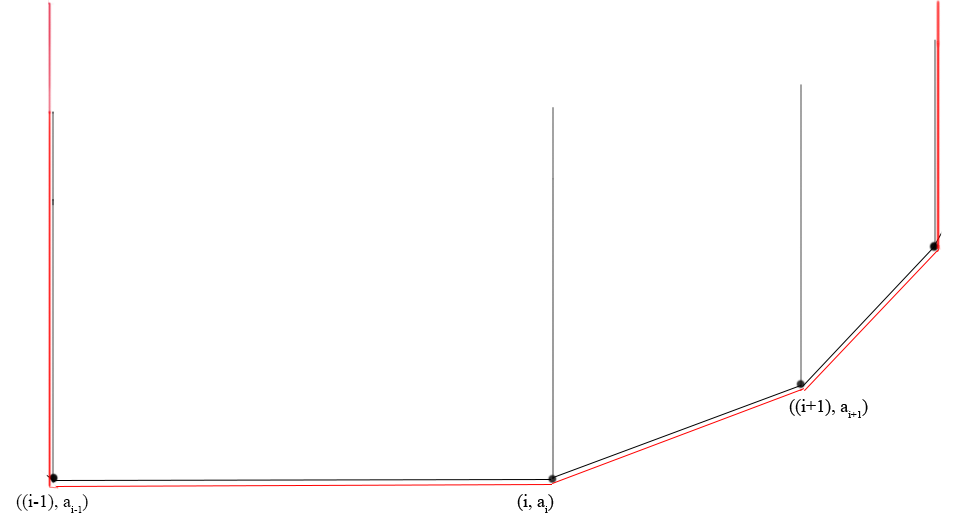
\includegraphics[scale=0.3]{mnogoug.png}}
\caption{Многоугольник Ньютона}
\end{figure}
\timestamp{47:55}
\begin{Definition}
	Тропическая рекуррентная последовательность $y$ \emph{минимальна}, если для любого $i\in Z$ нельзя уменьшить $y_i$, сохраняя все $y_j,j\neq i$ и принадлежащий $R_a$. Обозначим через $R_a^{(min)}$ множество тропических минимальных рекуррентных последовательностей, удовлетворяющих $a$.\; $R_a^{(min)}$ не обязательно тропическое линейное пространство, т.к. не всегда будет определена операция сложения векторов друг с другом или операция умножения вектора на скаляр.
\end{Definition}
Пример:

$a = (0,0,0)$. Тогда $y=\{\ldots , 0, 0, 1, 0, 0, 2,\ldots \}\in R_a$ - не минимальна:
можно уменьшить любую положительную координату, и все равно последовательность останется рекуррентной. Если мы такого не допускаем, т.е. вообще нельзя будет уменьшить ни один $y_i$, тогда последовательность называется минимальной.


Минимальные последовательности более интересны, т.к.
неминимальные будут иметь какие-то сторонние коэффициенты. Также, стоит подчеркнуть, что в силу того, что можно обозначить множество минимальных последовательностей, нетрудно заметить, что оно не обязательно является тропическим линейным пространством.


\timestamp{49:35}
\subsection{Периодические тропические рекуррентные последовательности}

Еще одна важная вещь ~--- это периодические
последовательности.


Сосредоточимся на ситуации,
когда многоугольник Ньютона является простым (Рис.3).

\begin{figure}[h!]
\center{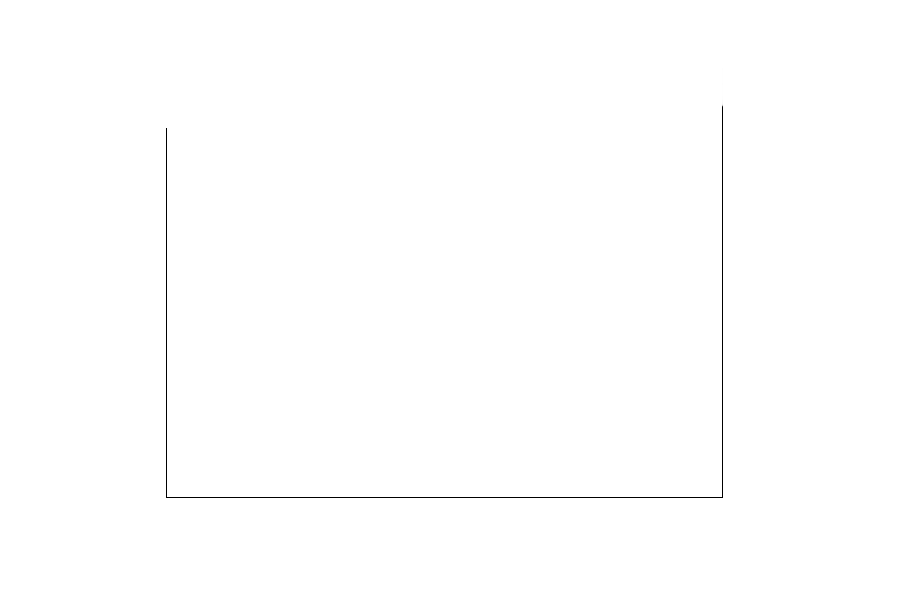
\includegraphics[scale=0.2]{prost.png}}
\caption{Простой многоугольник Ньютона}
\end{figure}

Он состоит, как мы говорили, из двух неограниченных рёбер, и мы предполагаем, что есть одно ограниченное ребро. Для простоты, можно считать, что оно горизонтальное, так как всегда плоскость можно повернуть. Таким образом, $a_0=a_n=0,\: a_i\geq 0,\: 1\leq i\leq n-1$. И в этой ситуации возникают периодические последовательности.

Что значит периодические рекуррентные последовательности? Это значит, что имеется какой-то период $d,$ т.е., если сдвинуть элемент последовательности на $d$, ничего не изменится: $y_i+d=y_i$.

Периодические рекуррентные последовательности в каком-то смысле тривиальны, потому что они соответствуют классическим последовательностям, а вот то, что не является периодическим ~--- это чисто тропический эффект. Поэтому то, что мы
дальше будем делать ~---- это изучать, когда имеются непериодические тропические минимальные рекуррентные последовательности, удовлетворяющие вектору $a$.

\timestamp{52:06}
\subsection{Случай: все точки лежат на ребре многоугольника Ньютона}

Обратим внимание на ситуацию, когда у нас есть ровно одно ребро многоугольника Ньютона. Это означает, что, во-первых, там есть две точки на конце, во-вторых, часть точек может лежать внутри многоугольника или на ребре. Далее в примерах мы, пока что, будем предполагать, что внутри точек вообще нет, все точки вектора $a$ лежат на ребре.


Однако сперва стоит сказать еще об одном геометрически полезном наблюдении. Как можно представить, что последовательность удовлетворяет вектору? Последовательность будем изображать $y_1,\: y_2,\: y_3,\: y_4$ и т.д. Если точнее, $(1,y_1),(2,y_2)$ - координаты точек этой последовательности. Она бесконечна в обе стороны. С другой стороны, есть вектор $a$. Для удобства отразим его, т.е. заменим координату $a_i$ на координату $-a_i$, и нарисуем точки.

Теперь, как можно геометрически сказать, что последовательность удовлетворяет вектору?  Это означает следующее: возьмем эту последовательность (Рис.4) и как-то ее сдвинем на любое целое число. И теперь начинаем двигать ее вверх, одновременно все точки.\\\\\\

\begin{figure}[h!]
\center{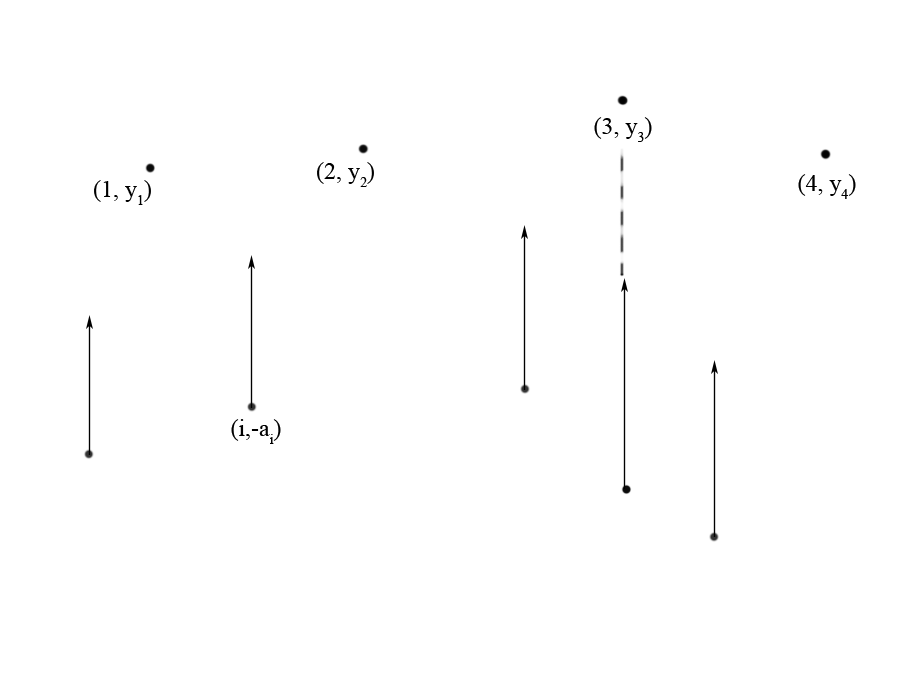
\includegraphics[scale=0.3]{toch.png}}
\caption{Геометрическая интерпретация условия, что $y$ является рекуррентной последовательностью, удовлетворяющей вектору $a$.}
\end{figure}

Как долго мы двигаем? До того момента, пока первая точка не упрётся в какой-то {\itshape y}.
Требование, чтобы $y$ была рекуррентной последовательностью, удовлетворяющую $a$, равносильно тому, чтобы при этом процессе движения, когда одна точка $a$ упёрлась в точку графика $y$, упёрлась и еще одна точка, т.е. по крайней мере две точки уперлись в график $y$. Это геометрическая интерпретация условия того, что $y$ является рекуррентной последовательностью, удовлетворяющей вектору $а$.

Пусть у нас есть последовательность, которая лежит, в первом случае, на ребре (Рис.5). Это означает, что у неё все координаты либо 0, либо бесконечность, т.е., если координата отсутствует ~--- это бесконечность, если она присутствует - это число. Обозначим через $I$, множество индексов, у которых точки присутствуют, например, 1, пропуск, 3, 4, 5, 6, то есть $I=\{1,3,4,5,6\}$. Пропуск означает, что $a_2=\infty$, а все остальные: $a_1=0=a_3=\ldots$ и т.д.


\begin{figure}[h!]
\center{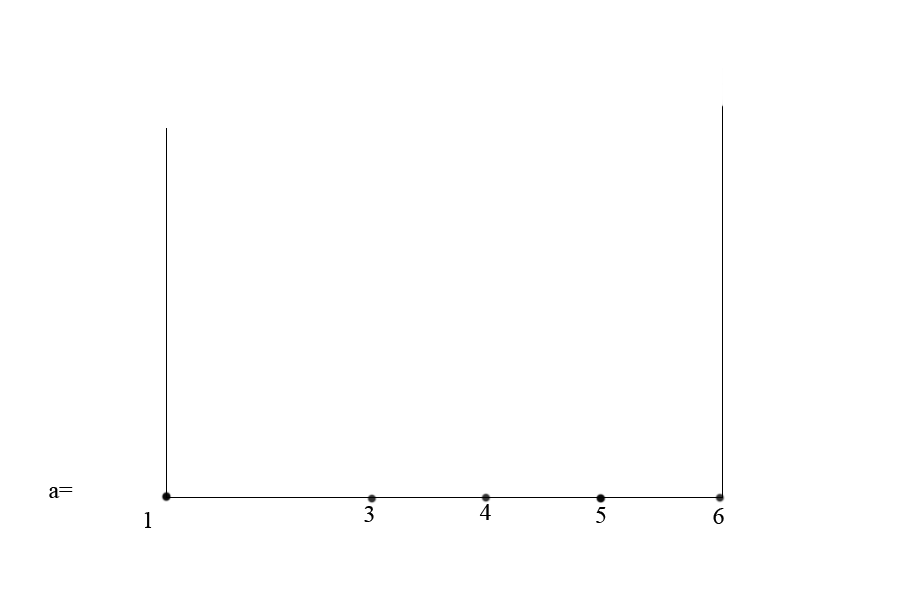
\includegraphics[scale=0.25]{recpos.png}}
\caption{Последовательность, лежащая на ребре.}
\end{figure}

В этой ситуации можно описать, когда имеются непериодические рекуррентные
последовательности, а именно, они имеются в том и только в том случае, если множество $I$ не образует арифметическую прогрессию. На данной картинке (Рис.5) непериодические последовательности образуются, из-за того, что двойка пропущена.\\
\timestamp{57:00}
\begin{Theorem}
	Все тропические минимальные рекуррентные последовательности являются периодическими, если множество I является арифметической прогрессией. В случае, когда эта прогрессия имеет разницу {\itshape d}, любая тропическая минимальная рекуррентная последовательность, удовлетворяющая {\itshape a}, имеет период {\itshape d}.
\end{Theorem}


Эту теорему нужно доказывать в обе стороны. В одну сторону её можно сформулировать так: если мы предположим, что множество $I$ образует арифметическую прогрессию, то почему тогда у нас других, кроме как периодических последовательностей, нет? (доказательство несложное, его лучше прочитать).

Доказательство в другую сторону можно проиллюстрировать. Допустим,
что у нас условие нарушено, т.е. $I$ не образует арифметическую прогрессию. Тогда покажем на картинке, используя наглядное представление, почему есть строгие непериодические последовательности.
 \emph{Пример:}

Рассмотрим простейший пример (Рис. 6). У нас всего три точки: 1, 3 и 4. Это множество $I$ не является арифметической прогрессией. Мы хотим построить непериодическую последовательность. Сперва начнем с периодической последовательности, $y_i$ - начальная последовательность, которая будет в каждой точке равна нулю. И теперь мы хотим ее <<испортить>>, сделать непериодической.

Как это сделать? Поместим наш вектор: 1,3 и 4 в любом месте. Будем сдвигать его вверх, и поднимем его до того, пока он не упрётся в начальную последовательность, а теперь сдвинем еще чуть-чуть, именно в этих точках (1,3,4), на одно и то же $\varepsilon$ - любое положительное число. Остальные не меняем.

\begin{figure}[h!]
\center{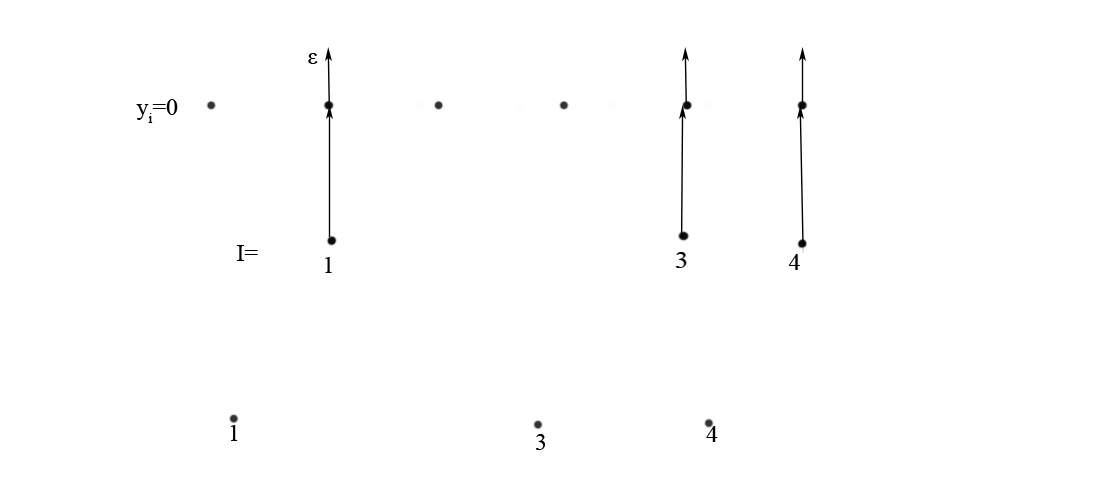
\includegraphics[scale=0.3]{period.png}}
\caption{Образование непериодической последовательности.}
\end{figure}

Нетрудно проверить, что то, что получится, будет снова удовлетворять нашему вектору, устроенному таким образом: $a_1=0=a_3=a_4$,
а все остальные коэффициенты вектора равны бесконечности.


Обобщим то, что мы проделали выше.

Дан вектор $a = (0,\infty,0,0)$, где $\infty$ означает пропуск.
Исходная последовательность была периодической $\{y_i=0\} _{i\in Z}$. Мы сделали из нее непериодическую (т.е. каждую точку  $y_i$ при $i\in\{1,3,4\}$ подняли вверх на положительное число $\varepsilon$) и получили непериодическую последовательность $y=\{\ldots,0,\varepsilon,0,\varepsilon,\varepsilon,0,\ldots\}$. Проверка будет заключаться в следующем:

\emph{Проверка:}
\begin{enumerate}
 \item
Согласно нашему представлению, мы должны взять вектор $a$, как-то сдвинуть и потом поднять его наверх так, чтобы он упёрся, по крайней мере, в двух точках $y$ при минимальном подъеме. Если мы поместим его так, как мы помещали, то это очевидно, потому что он в себя и упрется (Рис.7).\\\\\\\\

\begin{figure}[h!]
\center{\includegraphics[scale=0.4]{provfirst.png}}
\caption{Проверка. Первый случай.}
\end{figure}

Или $min\{a_1+y_1,\ a_3+y_3,\ a_4+y_4\}=min\{0+\varepsilon,\ 0+\varepsilon,\ 0+\varepsilon\}=\varepsilon$. Видно, что минимум достигся больше двух раз.
\item
Сдвинем вектор $a$ немного вправо. Он упрётся в двух точках: $y_2,\ y_5$  (Рис.8).
\begin{figure}[h!]
\center{\includegraphics[scale=0.4]{prov2.png}}
\caption{Проверка. Второй случай.}
\end{figure}

Или $min\{a_1+y_2,\ a_3+y_4,\ a_4+y_5\}=min\{0+0,\ 0+\varepsilon,\ 0+0\}=0$ - минимум достигся хотя бы два раза.
\end{enumerate}

Так будет и во всех остальных случаях, т.е. минимум будет достигаться хотя бы два раза. Это значит, что непериодическая последовательность  $y=\{\ldots,0,\varepsilon,0,\varepsilon,\varepsilon,0,\ldots\}$ удовлетворяет вектору $a$.

Но заметьте, что мы взяли какое-то произвольное место  в этой исходной последовательности из всех нулей и сдвинули. Мы можем так сделать в другом месте и так "испортить"\: ее бесконечно много раз, т.е. у нас получится сильная непериодичность (видно, что здесь получается очень много непериодических последовательностей).

Минимальность здесь будет автоматически,
потому что во всех случаях по крайней мере в две минимальные точки мы упираемся.

Видно, что последовательностей много. И возникает вопрос: а насколько их много? Это будет чуть дальше. То есть меру того,
насколько много последовательностей, мы опишем с помощью тропической энтропии.

\begin{Corollary}
	Если $P(a)$ имеет единственное ограниченное ребро (с точками {\itshape a}, возможно, из этого ребра), и точки на ребре не образуют арифметическую
	прогрессию, тогда существует тропическая непериодическая минимальная рекуррентная
	последовательность, удовлетворяющая $a$.\\
\end{Corollary}


То есть, если последовательность более общего вида: у нее не обязательно все точки лежат на ребре, а могут быть точки внутри, то в любом случае, если у нас на нижнем ребре была не арифметическая прогрессия, возникают непериодические последовательности.

\timestamp{71:45}
\subsection{ Случай: одно ограниченное ребро и точки на этом ребре образуют шаг арифметической прогрессии, равный двум}

В данном случае вопросов больше, чем ответов. Однако известен точный ответ, связанный с единственностью, а точнее два ответа. \\

Первый ~--- это когда
все точки лежат на одном ребре или их не существует. Мы уже сказали, что, если точки, лежащие на одном ребре, не образуют
арифметическую прогрессию, то есть непериодические последовательности, поэтому в этом случае будем рассматривать ситуацию, когда
точки, лежащие на ребре, образуют арифметическую прогрессию.

И второй случай, последний, на который есть ответ полностью, это когда точки, лежащие на ребре, образуют арифметическую прогрессию с разностью два, т.е. $P(a)$, с одним ограниченным ребром и точками$a$ на этом ребре, образующими арифметическую прогрессию с шагом 2. Предположим, что это будут нечетные точки, тогда про остальные (четные) мы ничего не знаем, их координата может даже равняться бесконечности (Рис.9).

\begin{figure}[h!]
\center{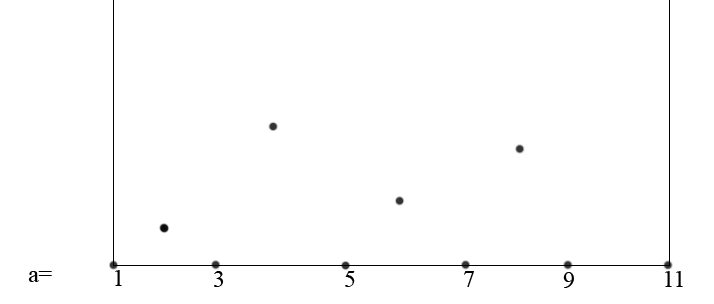
\includegraphics[scale=0.3]{nechet.png}}
\caption{Арифметическая прогрессия с шагом 2.}
\end{figure}


В этом случае ответ известен, он тоже очень простой.

Пусть все нечетные равны нулю($a_1=a_3=a_5=\ldots =a_n=0$), т.е. они лежат на нижнем ребре, а наоборот, четные ~--- положительные $a_{2i}>0,\:0\leq i<n/2$, иначе нарушаются условия арифметической прогрессии.

Тогда можно описать, когда все последовательности являются периодическими, а именно, точки, лежащие на остальных четных координатах, должны лежать на одном уровне, и только тогда все тропические рекуррентные последовательности будут являться периодическими (Рис.10).

\begin{figure}[h!]
\center{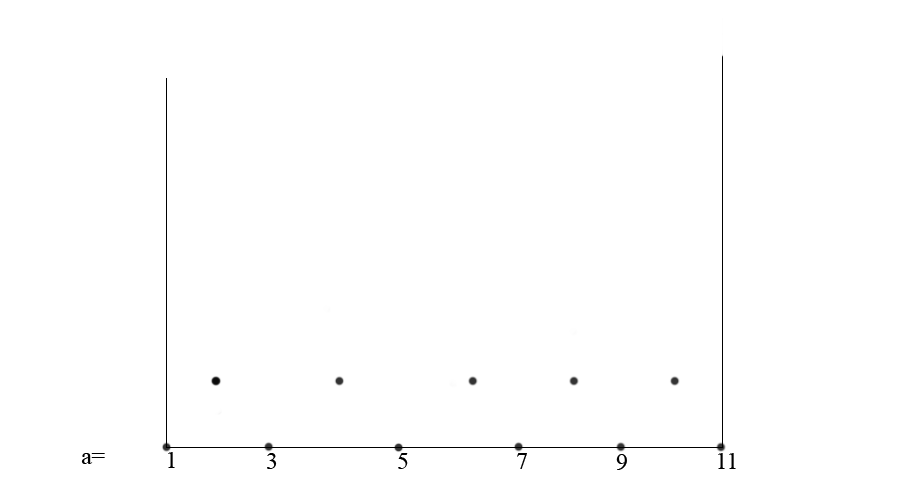
\includegraphics[scale=0.3]{uslovie.png}}
\caption{Периодическая тропическая рекуррентная последовательность}
\end{figure}


Опять же, доказательство в две стороны. В одну сторону формулировка будет такая: если выполненно условие, описанное выше, то все последовательности периодические, причем они
периодические с периодом 2.

Похожим способом <<испортим>> последовательность для доказательства условия в обратную сторону, сделаем ее непериодической.


Итак, дан вектор а. Для простоты он будет представлять из себя три точки, лежащие на одном уровне. Затем мы переворачиваем многоугольник Ньютона и записываем следующие точки. Условие нарушено - одна точка выбивается.(Рис. 11)

\begin{figure}[h!]
\center{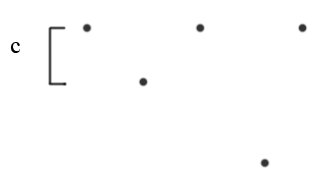
\includegraphics[scale=0.3]{podposl.png}}
\caption{Вектор а}
\end{figure}

Возьмем минимальное расстояние, пусть будет с, и возьмем теперь такое решение $y_0$ (Рис.12). То, что это будет решением легко проверить.

\begin{figure}[h!]
\center{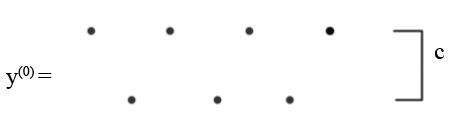
\includegraphics[scale=0.3]{resh.png}}
\caption{Решение}
\end{figure}
И теперь точно так же, как мы делали раньше, делаем следующее: начинаем двигать весь этот вектор вверх
параллельно, все точки одновременно, до той поры пока он не упрется в $y_0$ в четырех точках (отмечены крестиками на Рис. 13), и теперь, после
этого, мы еще чуть-чуть сдвинем эти точки на одно и то же $\varepsilon$ (Рис.13).

\begin{figure}[h!]
\center{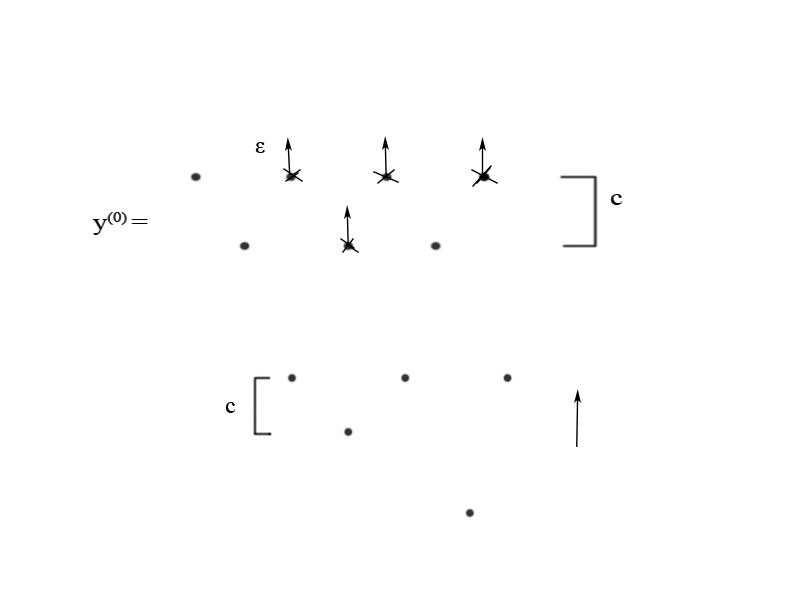
\includegraphics[scale=0.3]{last.png}}
\caption{Образование непериодичности}
\label{fig:image}
\end{figure}
Т.е. рецепт
очень похожий на то, что было раньше. Мы двигаем пока возможно, а после того, как упёрлись, мы еще продвигаем чуть-чуть, пока не <<доехала>> последняя точка (выбившаяся из арифметической прогрессии).

Обобщим наши рассуждения.
Был дан вектор $a=(a_1,a_2,a_3,a_4,a_5)$, где $a_1=a_3=a_5=0$, $a_2=c>0$  $(a_2=a1+c=0+c=c)$,  $a_4>c+\varepsilon$, т.е. $a=(0,c,0,a_4,0)$. И решение - периодическая последовательность $y^{(0)}=\{\ldots y_1,y_2,y_3,y_4,y_5,\ldots\}$, т.е. $y_1=y_3=y_5\ldots$, $y_2=y_4=y_6=\ldots$. Причем, $y_1=y_2+c$.

Мы снова ее "испортили" (двигали вектор $a$ параллельно вверх, пока он не уперся в $y^{(0)}$, а потом сдвинули $y^{(0)}$ на $\varepsilon$) и получили непериодическую последовательность: $y=\{y_2+c,\ y_2,\ y_2+c+\varepsilon,\ y_2+\varepsilon,\ y_2+c+\varepsilon,\ y_2,\ y_2+c+\varepsilon\}$. Проверим, удовлетворяет ли она подпоследовательности $a$.

\emph{Проверка:}
\begin{enumerate}
\item
Оставим $a$ на прежнем месте (Рис.14)

\begin{figure}[h!]
\center{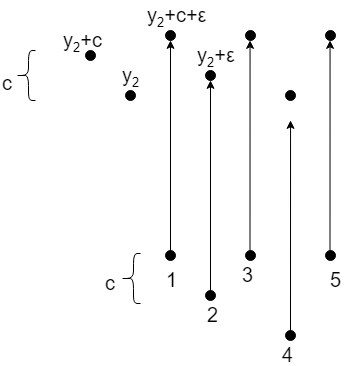
\includegraphics[scale=0.4]{pr1.png}}
\caption{Проверка. Первый случай.}
\end{figure}

Или $min\{a_1+y_2+c+\varepsilon,\ a_2+y_2+\varepsilon,\ a_1+y_2+\varepsilon+c,\ a_4+y_2, a_1+y_2+\varepsilon+c\}=min\{y_2+\varepsilon+c,\ y_2+\varepsilon+c,\ y_2+\varepsilon+c, a_4+y_2, y_2+\varepsilon+c\}=y_2+\varepsilon+c$ - минимум достигся больше двух раз.
\item
Сдвинем вектор $a$ немного вправо. Он упрётся в двух точках: $y_2,\ y_6$  (Рис.15).
\begin{figure}[h!]
\center{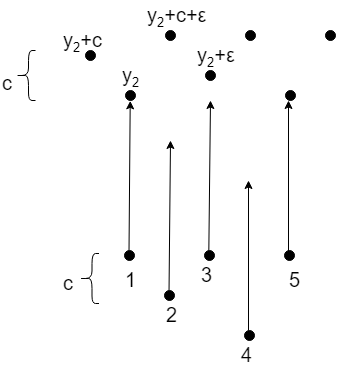
\includegraphics[scale=0.4]{pr2.png}}
\caption{Проверка. Второй случай.}
\end{figure}
Или $min\{a_1+y_2,\ a_2+y_2+\varepsilon+c,\ a_1+y_2+\varepsilon,\ a_4+y_2+\varepsilon+c, a_1+y_2\}=min\{y_2,\ y_2+\varepsilon+2c,\ y_2+\varepsilon, a_4+y_2+\varepsilon+c, y_2\}=y_2$ - минимум достигся хотя бы два раза. Так будет и во всех остальных случаях, т.е. минимум будет достигаться хотя бы два раза.
\end{enumerate}



И так можем аналогично этой конструкции сдвигать в любом другом месте. Поэтому получим континуальный запаc непериодических последовательностей.
\timestamp{77:35}
\subsection{Случай: одно ограниченное ребро и точки на этом ребре образуют шаг арифметической прогрессии, равный трем}

В данной ситуации полный ответ не выяснен. Здесь начинаются задачи, упражнения и прочее. Однако для этой ситуации совсем уж простейший случай известен. \\

\emph{Пример:}
\noindent Пусть $n=3, a_0 = a_3 = 0, a_1 > a_2 > 0$ (случай $a_2>a_1>0$ идентичен, случай $a_2=a_1>0$ имеет небольшой открытый вопрос), тогда многоугольник будет устроен так:

\begin{figure}[h]
\center{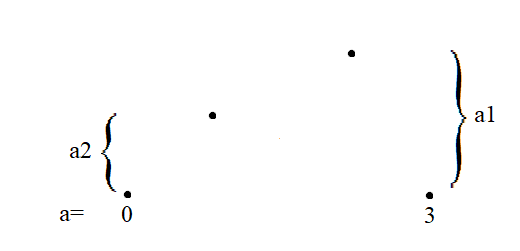
\includegraphics{Ris}}
\caption{Устройство многоугольника.}
\end{figure}

И спрашивается, когда в этой ситуации есть периодические последовательности? Ответ будет такой: все тропические минимальные рекуррентные последовательности, удовлетворяющие вектору $a$, являются периодическими, если $a_1 \le 2a_2$.

Теперь стоит сформулировать достаточно трудную проблему, к которой еще не придумана даже гипотеза. \\

\emph{Проблема.}
Как описать $a$, для которого все минимальные тропические рекуррентные последовательности, удовлетворяющие $a$, будут периодическими?\\


\emph{ Вопрос.}
Как описать вектора\\
$n=4, a_0=a_4=0, a_1>0, a_2>0, a_3>0$, для которых все минимальные тропические рекуррентные последовательности, удовлетворяющие $a$, будут периодическими?\\

Ответ на данный вопрос вполне можно получить, например, с помощью компьютера или вручную. Сама по себе задача является выполнимой для студентов младших курсов. Начать же можно с рассмотрения частных случаев. \\

Стоит уточнить, что в данной задаче по-прежнему рассматривается случай, когда многоугольник состоит всего из одного ребра. И так же данную задачу можно сделать более хитрой, если предположить, что некоторые точки будут лежать не выше ребра, а на нем.
\timestamp{84:50}
\subsection{ Алгоритм проверки существования тропических непериодических рекуррентных последовательностей}

\begin{Theorem}
	 Пусть $a = (a_0,\ldots, a_n) \in \mathbb{R}^{n+1}, a_0=a_n=0, 0 \le a_i \le M, 1 \le i \le n-1$( $P(a)$ имеет одно ограниченное ребро). Можно проверить существование тропических непериодических минимальных рекуррентных последовательностей, удовлетворяющих вектору $a$, в пределах сложности $M^{M^n}$.\\
\end{Theorem}


Данная теорема говорит о том, что есть алгоритм, благодаря которому мы можем узнать о существовании периодических последовательностей, удовлетворяющих $a$. Алгоритм имеет достаточно большую сложность и работает только в том случае, если все координаты $a$ конечные. Следовательно напрашиваются следующие вопросы по его улучшению:\\

\emph{Вопросы.} Как проверить существование, когда $a_i=\infty$ для некоторого $1 \le i \le n-1$ разрешены?\\
Возможно ли улучшить сложность? \\

Ответы на данные вопросы можно вполне получить, но сперва нужно изучить сам алгоритм.
\timestamp{85:50}
\section{Тропическая энтропия}


\subsection{Определение и происхождение}


Термин тропической энтропии вводится для измерения общего множества последовательностей.\\
\begin{Definition}
	Конечная последовательность $y = (y_0,\ldots, a_s) \in \mathbb{R}^{s}$ удовлетворяет $a=(a_0,\ldots, a_n)$, если для каждого $1 \le k \le s-n$ выполняется тропическое линейное уравнение: $min_{0\le i \le n}\{a_i + y_{k+i}\}$. $y$ будет называться минимальной, если для каждого $n<m\le s-n$ нельзя уменьшить $y_m$, сохраняя все $a_I$, $I\ne m$ и удовлетворяет $a$. \\
\end{Definition}


В данном случае ситуация даже упрощается, ведь мы будем рассматривать не бесконечные последовательности, а конечные (длины s). И точно так же дается определение минимальной последовательности (никакую координату нельзя безболезненно уменьшить).

И теперь мы попытаемся их все описать, так как это стало возможным из-за конечной длины пространства.

Обозначим через $D_s:=D_s(a) \in \mathbb{R}^{s}$(соответственно, $M_s:=M_s(a) \in \mathbb{R}^{s}$) набор из всех последовательностей (соответственно, минимальных последовательностей), удовлетворяющих $a$, и $d_s:=dimD_s, m_s:=dimM_s$. Обратим внимание на то, что $D_s, M_s$ конечное объединение многогранников. Это можно интуитивно понять, поскольку все тропические условия представляют из себя некоторые линейные неравенства и логические связки (и/или/отрицание). А из таких связок, кроме как конечное объединение многогранников, ничего не может получится.

Также, пусть $s=r+t$ и $p: \mathbb{R}^{s} \rightarrow \mathbb{R}^{r}$ (соответственно, $q: \mathbb{R}^{s} \rightarrow \mathbb{R}^{t}$) - это проекции на первые $r$ (соответственно, последние $t$) координат. Из этого следует достаточно простое утверждение, что $p(D_s) \subset D_r$, $q(D_s) \subset D_t$, $p(M_s) \subset M_r$, $q(M_s) \subset M_t$. Утверждение достаточно очевидно, так как, если у нас последовательность удовлетворяла рекуррентным соотношениям, то мы, проектируя, отбрасываем какие-то координаты, и то, что остается, все равно будет удовлетворять рекуррентным соотношениям. То же самое и с минимальностью.

Таким образом, $d_s \le d_r + d_t, m_s \le m_r + m_t$, то есть суммарная размерность этого множества не будет превосходить суммы размерностей проекций на первые и на последние координаты. Проверка этого - упражнение из линейной алгебры. В свою очередь такие последовательности, удовлетворяющие условиям выше, называются полуаддитивными. Из эргодической же теории мы знаем, что если последовательность полуаддитивна, то корректно определены пределы: $H(a):= lim_{s\to\infty}\frac{d_s}{s} > h(a):= lim_{m\to\infty}\frac{m_s}{s} \ge 0$, которые в свою очередь и называются тропической энтропией и, соответственно, тропической минимальной энтропией. Существование самого предела называется эргодической леммой.

Понятие же энтропии впервые возникло из физики, а точнее из термодинамики. Его, скорее всего, придумал Больцман еще в 19 веке. Оно описывало степень неопределенности движения молекул газа. Также многие слышали про второе начало термодинамики, о том, что энтропия возрастает. Это означает, можно сказать на житейском языке, что, если мы ничего не делаем, то хаос будет возрастать. И то же самое научным языком - в замкнутой системе возрастает энтропия. Понятие энтропии же перекачивало из физики в математику, в теорию информации, где стало одним из фундаментальных понятий. Сама по себе энтропия - мера неопределенности.

Также, хочется сказать, что энтропия - число неотрицательное, и даже более того - сверху ограничено строго единицей. При энтропии, равной нулю, наблюдается полный порядок, никакого хауса нет, все однозначно. Это примерно, очень грубо, соответствует однозначному определению следующей координаты в рекуррентной тропической последовательности. А когда энтропия положительна, тогда есть хаос, есть неопределенность и есть, что считать.
\timestamp{92:50}
\subsection{Границы тропической энтропии}


\emph{Утверждение.} $H(a) \le 1 - 1/n$\\

Из этого утверждения видно, что энтропия ~--- число положительное и её можно даже чуть получше ограничить.\\

\emph{Пример:}
Пусть $a = (0,0,\ldots,0) \in \mathbb{R}^{n+1}.$ Тогда $H(a) = 1 - 2/(n+1), h(a) = 0.$ \\

В данном примере энтропия, по-видимому, будет самая большая. Малая энтропия соответственно будет равна нулю.

На основе этого примера можно сформулировать следующую гипотезу:\\

\emph{ Гипотеза.}  $H(a) \le 1 - 2/(n+1).$\\

Мы предполагаем, что оценку, приведенную в утверждении выше, можно улучшить данным соотношением. Любой ответ по данной проблеме был бы очень хорошей работой.\\

Следующие теоремы говорят о том, что энтропия очень часто положительная, а равенство нулю достигается совсем в редких случаях.\\
\timestamp{93:45}
\begin{Theorem}
	Если $P(a)$ имеет $\ge$ 3 точек на одном из своих ребер,тогда $H(a) \ge 1/4$.
\end{Theorem}

\begin{Theorem}
 Если $P(a)$ имеет одно ограниченное ребро и точек по крайней мере 3, то тогда $H(a) \ge 1/6$.\\
\end{Theorem}



Вследствие этого напрашивается вопрос. Бывает ли, чтобы энтропия равнялась нулю? Такая ситуация возможна:\\

\emph{Пример:}
Если точки, принадлежащие $a \in \mathbb{R}^{n+1}$, являются вершинами $P(a)$, тогда $H(a) = 0$.\\

То есть в многоугольнике Ньютона все точки лежат только в вершинах и нигде больше (Рис. 17).

\begin{figure}[h]
\center{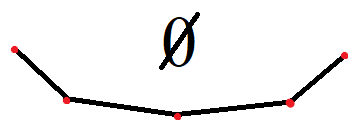
\includegraphics{Ris1}}
\caption{Устройство многоугольника.}
\end{figure}

Также хочется добавить, что в данной ситуации каждый последующий член последовательности будет определяться малым количеством способов (но не единственным). Но энтропия все равно будет равняться нулю, так как энтропия -- достаточно грубая характеристика, и она не учитывает малое количество способов.

Помочь в понимании этого может представленный ниже рисунок.

\begin{figure}[h]
\center{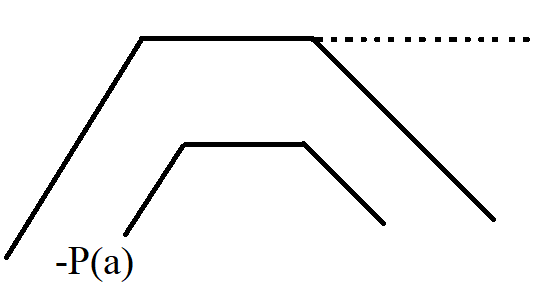
\includegraphics[scale=0.5]{Ris2}}
\caption{Устройство многоугольника и решения.}
\end{figure}

То есть, переворачивая наш многоугольник Ньютона, мы можем понять, какие у последовательности будут решения. И становится видно (на последнем ребре), что мы можем, растягивая наш многоугольник, продлить верхнюю грань решения, и все останется верным. Однако мы можем загнуть ребро и перейти к третьей грани, и все также остаётся верным. Отсюда и следует, что энтропия равна нулю, в силу малого количества возможностей.

Однако все равно ставится проблема, а когда энтропия вообще равна нулю?\\

\emph{ Проблема.}  Как описать $a$, для которых $H(a)=0$?.\\

Хотелось бы свести эту проблему к решению предыдущей задачи и сказать, что энтропия равна нулю тогда, когда мы имеем малое количество возможностей. Это представляет из себя хорошую задачу на исследование.\\

\emph{Упражнения.}

1) Вычислить $H(a)$ для $a = (0,0,2,1);$

2) Для каких b $H(a) = 0$, где $a = (0,0,b,1)?$
\timestamp{98:25}
\subsection{Границы минимальной тропической энтропии}


Гипотетически, мы предположили, что энтропия равна нулю, когда все точки лежат в вершинах многоугольника Ньютона. Вследствие этого напрашивается следующий вопрос. А в каких случаях минимальная тропическая энтропия равна нулю? Возьмем пример, который мы уже рассматривали:\\

\emph{ Пример} Пусть $a=(0,a_1,a_2,0), a_2>2a_1>0.$ Мы уже упоминали, что в данном случае есть непериодические последовательности. И в этом примере $h(a) \ge 1/9$. Если же не было непериодических последовательностей, то есть $2a_1 \ge a_2>a_1>0$, тогда $h(a) = 0$.\\

Из этого примера вытекают следующие проблемы.\\

\emph{ Проблемы.}

(1) Для $a$ с $P(a)$, имеющим только одно ограниченное ребро, является ли верным то, что $h(a) = 0$, только в том случае, если все тропические минимальные рекуррентные последовательности, удовлетворяющие $a$, периодические?

(2) Пусть $a \in (\mathbb{R} \cup \{ \infty \})^n$. Верно ли, что функция $d_s$ линейна по s с ведущим коэффициентом $H(a)$ для s из каждой арифметической прогрессии с различным $n$?\\

По поводу второй проблемы, хочется отметить, что во всех примерах это условие выполняется, и хотелось бы, чтобы это выполнялось всегда.\\

И еще один вопрос, который вполне можно сделать. Можно сказать, что этот вопрос параллелен вопросу о вычислении непериодичности последовательности. Мы проверяем, что малая энтропия равна нулю только в случае, если все последовательности периодические.\\

\bfseries Вопрос. \mdseries Для каких $a_1,a_2,a_3>0 \; h(a) =0$, где $a=(0,a_1,a_2,a_3,0)$?.
\end{document}
